\documentclass[11pt,a4paper]{article}
\usepackage[T1]{fontenc}
\usepackage[margin=2.3cm]{geometry}
\usepackage{amsmath,amssymb}
\usepackage{graphicx}
\usepackage[dvipsnames]{xcolor}
\usepackage{enumitem}
\usepackage[colorlinks=true,linkcolor=blue,urlcolor=blue]{hyperref}
\setlength{\parskip}{0.6em}
\setlength{\parindent}{0pt}
\begin{document}

\begin{center}{\LARGE\bfseries openseasons}\\[0.4em]{\large Why we have day, night, seasons and Moon phases: geometry you can compute.}\\[0.2em]\small PAN IIT OSS explainer \textbullet{} secondary school to diploma / undergraduate (levels 3-5)\end{center}

\section*{Why this exists}
Day and night, seasons and Moon phases are the first astronomy that every child meets, and the most often misunderstood. This explainer rebuilds them from a few vectors and angles, so each claim can be checked by a number.

\section*{The end goal}
Explain day, night, seasons and Moon phases with geometry. The end goal is to explain day, night, seasons and Moon phases with geometry, and to be able to compute them for any place and date. The same vector methods are used in solar-energy design and in satellite and telescope pointing.

\section*{How the three sessions build up}
\begin{enumerate}[nosep]
\item \textbf{Session 1: Spin, tilt and the lit half} (Level 1, conceptual interactive model, 60 min).
\item \textbf{Session 2: The tilted axis as a vector} (Level 2, mathematical engineering model, 75 min).
\item \textbf{Session 3: Simulating the Moon} (Level 3, simulation and validation, 90 min).
\end{enumerate}

\section{Session 1: Spin, tilt and the lit half}

\subsection*{A. Real-world problem}
In early January the Earth is closest to the Sun, yet it is winter in India, Europe and North America and summer in Australia and Argentina. Why do we have day and night, why is June hot and December cold at your latitude, and why does the Moon grow from a thin crescent to a full disc? Three simple geometrical ideas explain all of it, and you can test each with a number.

\subsection*{B. Concept and theory}
A place is in daylight when its up direction points towards the Sun: the dot product of the up vector and the Sun direction is positive. As the Earth spins (15 degrees per hour) the place goes round a circle of latitude, half of it in light for a tilt of zero, so every day has 12 hours. The axis is tilted by 23.4 degrees from the line at right angles to the orbit and keeps pointing the same way in space. So the latitude where the Sun is overhead (the declination d) swings between +23.4 and -23.4 degrees over a year. At noon the Sun height is 90 - \textbar{}latitude - d\textbar{}. The Earth-Sun distance changes only from 147.1 to 152.1 million km, smallest on about 4 January, and it is the same for both hemispheres while their seasons are opposite. The Moon is always lit on one half by the Sun; the elongation D (angle Sun-Earth-Moon) decides how much of that half faces us, k = (1 - cos D) / 2.

\begin{itemize}[nosep]
\item tilt: tilt of the Earth's axis from the orbit normal (23.4) (degrees)
\item lat: latitude of a place (north positive) (degrees)
\item d: declination: latitude where the Sun is overhead (degrees)
\item n: day of the year (1 January = 1) (days)
\item r: Earth-Sun distance (million km)
\item D: elongation Sun-Earth-Moon (degrees)
\item k: bright fraction of the Moon's disc (no unit)
\end{itemize}

\begin{equation*}
\hat n\cdot\hat s>0\ \Longleftrightarrow\ \text{daylight}
\end{equation*}

\begin{equation*}
\sin d=\sin(\text{tilt})\,\sin\!\left(\frac{2\pi(n-80)}{365.25}\right)
\end{equation*}

\begin{equation*}
\text{noon height}=90^\circ-|\text{lat}-d|
\end{equation*}

\begin{equation*}
r=149.6\left(1-0.0167\cos\frac{2\pi(n-4)}{365.25}\right)\ \text{million km}
\end{equation*}

\begin{equation*}
k=\frac{1-\cos D}{2}
\end{equation*}

\begin{center}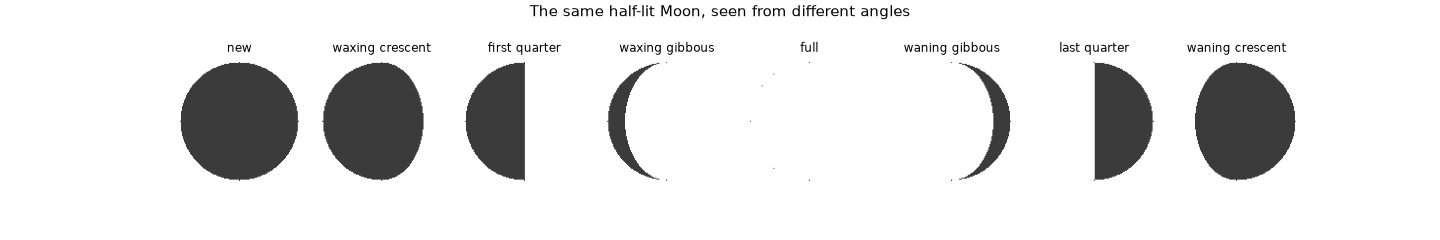
\includegraphics[width=0.85\linewidth]{figures/s01_moon_phases.png}\\\small The same half-lit Moon at eight elongations, computed from a dot product.\end{center}

\subsection*{E. Worked example}
Find the noon Sun height at latitude 40 N on 21 June and on 21 December, using a tilt of 23.4 degrees.
\begin{enumerate}[nosep]
\item On 21 June the Sun is overhead at the declination d = +23.4 degrees.
\item Height = 90 - \textbar{}40 - 23.4\textbar{} = 90 - 16.6 = 73.4 degrees.
\item On 21 December d = -23.4 degrees, so height = 90 - \textbar{}40 + 23.4\textbar{} = 90 - 63.4 = 26.6 degrees.
\item The model code gives the same two numbers, and also the day length 14.84 h in June and 9.16 h in December.
\end{enumerate}
\textbf{Answer.} 73.4 degrees in June and 26.6 degrees in December: a swing of 46.8 degrees, which is twice the tilt.

\subsection*{F. Questions}
\begin{enumerate}[nosep]
\item \textbf{Conceptual.} A friend says that summer is when the Earth is closest to the Sun. Give two pieces of evidence that this is wrong.
\item \textbf{Numerical.} Find the noon Sun height at 60 N on 21 June and on 21 December with tilt 23.4 degrees.
\item \textbf{Graph and simulation interpretation.} In the noon-height graph for 40 N and 40 S, at about which days do the two curves cross, and what is the height there?
\item \textbf{Design and optimisation challenge.} Design: you want a place where the noon Sun is never lower than 45 degrees at any time of the year. With tilt 23.4 degrees, what is the largest latitude (north or south)?
\end{enumerate}

\section{Session 2: The tilted axis as a vector}

\subsection*{A. Real-world problem}
A solar-farm planner needs the length of the day, the noon Sun height and the daily sunlight for a latitude on any date of the year, and a colleague insists that the seasons come from the distance to the Sun, which changes by 5 million km. Can you build the numbers from vectors, verify them against an independent calculation and show, with data, which of the two causes wins?

\subsection*{B. Concept and theory}
Use axes with x towards the March equinox direction, y along the orbit plane and z at right angles to it. The spin axis keeps its direction in space: a = (0, sin T, cos T), with T = 23.44 degrees. The direction from the Earth to the Sun at ecliptic longitude lam is s = (cos lam, sin lam, 0). The latitude where the Sun is overhead has up direction s, and latitude is measured from the equator, so its sine is the dot product with the axis: sin d = s . a = sin T sin lam. This peaks at d = T at the June solstice (lam = 90). For a place at latitude phi, daylight needs cos(phi) cos(d) cos(h) + sin(phi) sin(d) \textgreater{} 0, which gives the sunrise hour angle cos(H0) = -tan(phi) tan(d) and a day of 2 H0 / 15 hours; a value of the right side of at least 1 means polar night and of at most -1 means polar day. The polar limit is the latitude 90 - T. The noon height is 90 - \textbar{}phi - d\textbar{}. The sunlight falls as 1/r\textasciicircum{}2; r goes from 0.98329 to 1.01671 AU (147.1 to 152.1 million km), so sunlight at perihelion is (152.1/147.1)\textasciicircum{}2 = 1.069 times that at aphelion. In one day the Earth turns 360 degrees relative to the stars but also moves 360/365.2422 = 0.9856 degrees round the Sun, so the solar day needs that much extra spin: 235.9 s.

\begin{itemize}[nosep]
\item T: tilt of the axis (degrees)
\item lam: ecliptic longitude of the Sun (0 at March equinox) (degrees)
\item a, s: unit vectors: spin axis and direction to the Sun (no unit)
\item d: declination = subsolar latitude (degrees)
\item phi: latitude of a place (degrees)
\item H0: sunrise hour angle (degrees)
\item r: Earth-Sun distance (AU (1 AU = 149.598 million km))
\item S0: sunlight at 1 AU on a surface facing the Sun (1361) (W/m\textasciicircum{}2)
\item Q: mean daily sunlight on horizontal ground (top of the atmosphere) (W/m\textasciicircum{}2)
\end{itemize}

\begin{equation*}
\sin d=\hat s\cdot\hat a=\sin T\,\sin\lambda
\end{equation*}

\begin{equation*}
\cos H_0=-\tan\phi\,\tan d,\qquad \text{day length}=\frac{2H_0}{15^\circ}\ \text{h}
\end{equation*}

\begin{equation*}
Q=\frac{S_0}{\pi r^2}\left(H_0\sin\phi\sin d+\cos\phi\cos d\sin H_0\right)
\end{equation*}

\begin{equation*}
\frac{S_{\text{peri}}}{S_{\text{aph}}}=\left(\frac{r_{\text{aph}}}{r_{\text{peri}}}\right)^2
\end{equation*}

\begin{equation*}
\frac{1}{T_{\text{solar}}}=\frac{1}{T_{\text{sidereal}}}-\frac{1}{T_{\text{year}}}
\end{equation*}

\begin{center}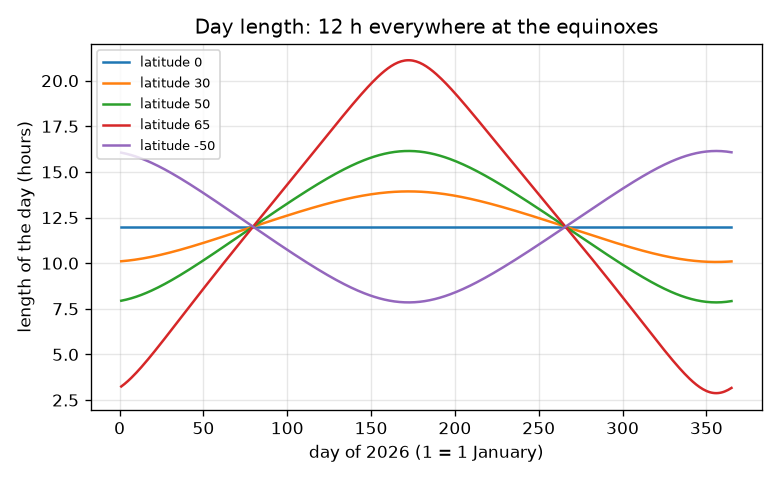
\includegraphics[width=0.85\linewidth]{figures/s02_day_length.png}\\\small Day length against date at five latitudes: 12 hours everywhere at the equinoxes.\end{center}

\subsection*{E. Worked example}
Find the declination, day length and noon Sun height at latitude 40 N on the June solstice (tilt 23.44 degrees).
\begin{enumerate}[nosep]
\item At the solstice lam = 90 degrees, so sin d = sin 23.44 sin 90 = 0.3978 and d = 23.44 degrees.
\item cos H0 = -tan 40 tan 23.44 = -0.8391 * 0.4336 = -0.3638, so H0 = 111.33 degrees.
\item Day length = 2 * 111.33 / 15 = 14.84 hours.
\item Noon height = 90 - \textbar{}40 - 23.44\textbar{} = 73.44 degrees.
\item Check: counting the part of a latitude circle with a positive dot product gives the same 14.84 hours, and the maximum of that dot product gives the same 73.44 degrees.
\end{enumerate}
\textbf{Answer.} d = 23.44 degrees, day length 14.84 hours, noon height 73.44 degrees.

\subsection*{F. Questions}
\begin{enumerate}[nosep]
\item \textbf{Conceptual.} Explain in words why the dot product of the Sun direction with the spin axis is the sine of the latitude where the Sun is overhead.
\item \textbf{Numerical.} Find the day length at 50 N on the June solstice (d = 23.44 degrees) and the noon Sun height.
\item \textbf{Graph and simulation interpretation.} From the sunlight graph for 45 N and 45 S, why is the southern summer peak (510 W/m\textasciicircum{}2) higher than the northern (478 W/m\textasciicircum{}2)? Does it explain the seasons?
\item \textbf{Design and optimisation challenge.} Design: an amateur astronomer wants to keep a star centred. How much earlier does a star rise by the clock each solar day, and how much earlier after 30 days? Why does the sky of a season change?
\end{enumerate}

\section{Session 3: Simulating the Moon}

\subsection*{A. Real-world problem}
A school wants a printed Moon calendar for 2026 and a table of day length, noon Sun height and Moon phase for its latitude. People also ask why there is not an eclipse every month and whether the Moon's phases are the Earth's shadow. Can you simulate the angles, compare with the almanac, state the error and answer both questions with numbers?

\subsection*{B. Concept and theory}
The phase angle i is the angle at the Moon between the directions to the Sun and to the Earth. The bright fraction is k = (1 + cos i) / 2: 0 at new (i = 180), 0.5 at the quarters (i = 90) and 1 at full (i = 0). Because the Sun is 389 times farther than the Moon, i is almost exactly 180 - D, where D is the elongation. The Moon needs 27.32 days (sidereal month) to return to the same star, but the Earth has moved on, so the Moon must go further to catch up with the Sun; in one day the cycle gains 1/T\_sid - 1/T\_year, giving 1/T\_syn = 1/T\_sid - 1/T\_year and T\_syn = 29.5306 days. The elongation grows 360/29.5306 = 12.19 degrees a day (0.508 degrees an hour). A Moon on the celestial equator rises when its hour angle is -90 degrees; the Sun's hour angle grows 15 degrees an hour and D is growing, so the delay between moonrises is 12.19 / (15 - 0.508) = 0.841 h = 50.5 minutes, equal to 24 h * 29.53 / 28.53 - 24 h. The Moon's orbit is tilted 5.145 degrees to the Earth's, so at new or full its ecliptic latitude is asin(sin(5.145) sin(u)), where u is its angle from the node. An eclipse is possible only if the latitude is below about 1.48 degrees (the two angular radii plus the Moon's parallax), which happens for 2 asin(1.48 / 5.145) / pi = 18.5 percent of new Moons if u is random. Finally the Earth's umbra has radius 4600 km at the Moon's distance, 2.65 Moon radii, and lies on the line from the Sun through the Earth.

\begin{itemize}[nosep]
\item D: elongation Sun-Earth-Moon (degrees)
\item i: phase angle Sun-Moon-Earth (degrees)
\item k: bright fraction of the disc (no unit)
\item T\_sid, T\_syn, T\_year: sidereal month 27.321662, synodic month, sidereal year 365.25636 (days)
\item u: Moon's angle from a node of its orbit (degrees)
\item beta: Moon's ecliptic latitude (degrees)
\item epsilon: tilt of the Moon's orbit, 5.145 (degrees)
\item delay: extra time between moonrises (minutes)
\end{itemize}

\begin{equation*}
k=\frac{1+\cos i}{2},\qquad i\approx 180^\circ-D
\end{equation*}

\begin{equation*}
\frac{1}{T_{\text{syn}}}=\frac{1}{T_{\text{sid}}}-\frac{1}{T_{\text{year}}}
\end{equation*}

\begin{equation*}
\text{delay}=\frac{360/T_{\text{syn}}}{15-360/(24\,T_{\text{syn}})}\ \text{h}
\end{equation*}

\begin{equation*}
\beta=\arcsin\!\left(\sin\epsilon\,\sin u\right),\qquad P=\frac{2}{\pi}\arcsin\frac{\beta_{\max}}{\epsilon}
\end{equation*}

\begin{equation*}
R_{\text{umbra}}=R_E-d\,\frac{R_S-R_E}{D_{\text{Sun}}}
\end{equation*}

\begin{center}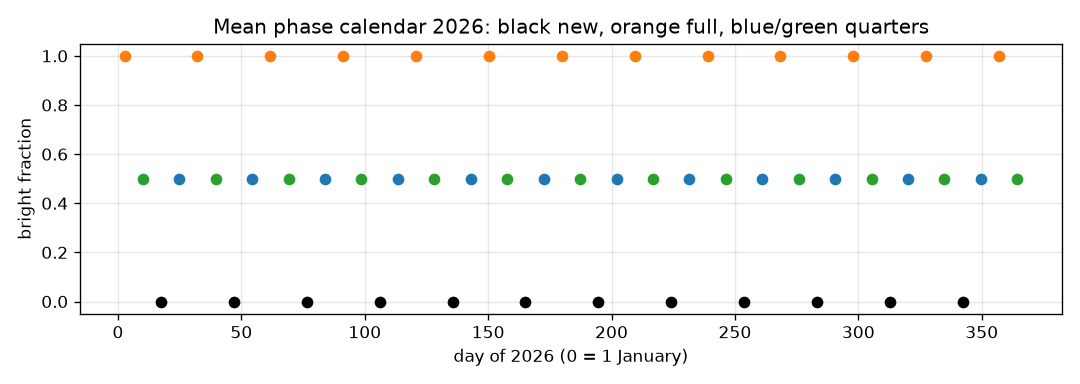
\includegraphics[width=0.85\linewidth]{figures/s03_calendar_2026.png}\\\small Mean-motion phase calendar for 2026 from the simulation.\end{center}

\subsection*{E. Worked example}
Derive the synodic month from a sidereal month of 27.321662 days and a sidereal year of 365.25636 days.
\begin{enumerate}[nosep]
\item 1 / 27.321662 = 0.036601 per day and 1 / 365.25636 = 0.002738 per day.
\item The difference is 0.033864 per day.
\item T\_syn = 1 / 0.033864 = 29.5306 days.
\item The accepted mean synodic month is 29.530589 days: the model is within 0.001 day.
\end{enumerate}
\textbf{Answer.} T\_syn = 29.5306 days, about 29 days 12 hours 44 minutes.

\subsection*{F. Questions}
\begin{enumerate}[nosep]
\item \textbf{Conceptual.} Explain why the Earth's shadow cannot be the cause of the Moon's phases, using the shadow size and the geometry at first quarter.
\item \textbf{Numerical.} At what Moon age is exactly 25 percent of the disc bright, in the first half of the month?
\item \textbf{Graph and simulation interpretation.} From the moonrise graph, when does the Moon rise on the night of new Moon and on the next night? What does the slope tell you?
\item \textbf{Design and optimisation challenge.} Design: a model Moon orbit has a tilt such that one new Moon in three would be near a node. What tilt is that, and what does it say about eclipses in a world with such a tilt?
\end{enumerate}

\section{Real-world mini-project}
\textbf{A year table for your latitude.} Choose a latitude (we use 60 degrees north as the example; use your own town too). With \texttt{year\_table} from Session 3, build the table of day length, noon Sun height and Moon phase for the 21st of every month of 2026, and add the rows for the nearest full Moon dates.

\section{The path ahead}
\begin{enumerate}[nosep]
\item \textbf{Session 4: A truer Moon calendar.} A phase calendar that adds the largest periodic terms.
\item \textbf{Session 5: Moonrise for a real place.} A moonrise calculator for a latitude, using the Moon's declination from the 5.145 degree tilt.
\item \textbf{Session 6: The analemma.} A figure-eight of the Sun's position at a fixed time through the year.
\item \textbf{Session 7: Kepler orbit instead of a series.} An Earth-Sun distance and speed from the eccentricity 0.0167 by a numerical solver.
\item \textbf{Session 8: Animate the whole sky.} A looping animation like the Target, with the Earth, the day-length curves and the Moon disc together.
\end{enumerate}

\section{Answers and hints}

\subsection*{Session 1}
\begin{enumerate}[nosep]
\item \textbf{Conceptual.} Hint: Compare the date of the smallest distance with the northern season, and think of the southern hemisphere on the same day. Solution: The smallest distance (147.1 million km) is on about 4 January, in northern winter, and the largest (152.1) is in early July, in northern summer. Also on one date the whole Earth is at one distance, but the two hemispheres have opposite seasons; on 4 January the noon Sun at 40 N is only 27.5 degrees high but at 40 S it is 72.5 degrees high. A cause that is the same for both cannot make them different.
\item \textbf{Numerical.} Hint: Height = 90 - \textbar{}lat - d\textbar{} with d = +23.4 and -23.4. Solution: June: 90 - (60 - 23.4) = 53.4 degrees. December: 90 - (60 + 23.4) = 6.6 degrees. Sanity check: the Sun is lower at higher latitude in both seasons, and the June value is higher than the December one.
\item \textbf{Graph and simulation interpretation.} Hint: They cross when both hemispheres get the same Sun, which means the Sun is over the equator. Solution: They cross at the equinoxes, around day 80 (20 March) and day 263 (23 September), where d is close to 0 and both heights are 90 - 40 = 50 degrees.
\item \textbf{Design and optimisation challenge.} Hint: The lowest noon Sun happens in the winter of that hemisphere, 90 - lat - 23.4. Solution: We need 90 - lat - 23.4 \textgreater{}= 45, so lat \textless{}= 21.6 degrees. Within 21.6 degrees of the equator the noon Sun is always at least 45 degrees high. The trade-off: such places have almost no change in day length either, so they have little seasonal variation; the model ignores clouds and the atmosphere.
\end{enumerate}

\subsection*{Session 2}
\begin{enumerate}[nosep]
\item \textbf{Conceptual.} Hint: At the subsolar point the up direction is the Sun direction. How is latitude related to the angle between up and the axis? Solution: Latitude is the angle above the equator, and the equator is the plane at right angles to the axis. For a unit up vector u, the dot product u . a = cos(angle from the axis) = sin(latitude). At the subsolar point u is the unit Sun direction s, so sin d = s . a. Since s = (cos lam, sin lam, 0) and a = (0, sin T, cos T), the dot product is sin T sin lam.
\item \textbf{Numerical.} Hint: cos H0 = -tan 50 tan 23.44, then day = 2 H0 / 15. Solution: cos H0 = -1.1918 * 0.4336 = -0.5168, so H0 = 121.1 degrees and the day is 2 * 121.1 / 15 = 16.15 hours. The noon height is 90 - (50 - 23.44) = 63.44 degrees. Sanity check: longer than 14.84 h at 40 N, as expected at higher latitude in summer.
\item \textbf{Graph and simulation interpretation.} Hint: Compare the Earth-Sun distance in January and July. Solution: In January the Earth is nearer the Sun (147.1 against 152.1 million km), so the 1/r\textasciicircum{}2 factor, up to 1.069, raises the southern peak. But the winter-to-summer change in each hemisphere (126 to 478 W/m\textasciicircum{}2 in the north) is a factor of about 3.8, far larger than 1.069, and its sign is opposite in the two hemispheres. So the tilt makes the seasons and distance only modifies them by a few percent.
\item \textbf{Design and optimisation challenge.} Hint: Use the 235.9 s per day difference between solar and sidereal days. Solution: A star rises 235.9 s (3 min 56 s) earlier each day. After 30 days: 30 * 235.9 s = 7077 s = 118 minutes, nearly 2 hours. So the stars you see at 9 pm shift: after half a year they are 12 hours different, which is why the constellations change with the seasons.
\end{enumerate}

\subsection*{Session 3}
\begin{enumerate}[nosep]
\item \textbf{Conceptual.} Hint: Where is the shadow, and where is the Moon at quarter? Solution: The Earth's shadow points straight away from the Sun, and at the Moon's distance its dark core has a radius of about 4600 km. At first quarter the Moon is 384400 km sideways from the line through the Sun and the Earth, 84 times the shadow radius, far outside it. The shadow can touch the Moon only within 0.94 degrees of full Moon (about 3.7 hours a month) and then only if the Moon is also near a node. So the shadow causes lunar eclipses, not phases.
\item \textbf{Numerical.} Hint: Solve (1 - cos D) / 2 = 0.25, then age = D / 360 * 29.53. Solution: cos D = 0.5, so D = 60 degrees and age = 60 / 360 * 29.53 = 4.92 days. Sanity check: between new Moon (0) and first quarter (7.38 days).
\item \textbf{Graph and simulation interpretation.} Hint: Read the first two points and subtract. Solution: At new Moon it rises at about 6.2 h (just after sunrise) and the next day at about 7.05 h. The slope is 0.84 h = 50.5 minutes per day: each day the Moon has moved 12.19 degrees further east and the Earth must turn that much more to bring it up.
\item \textbf{Design and optimisation challenge.} Hint: Set 2 asin(1.4763 / tilt) / pi = 1/3. Solution: asin(x) = pi/6 so x = 0.5 and tilt = 1.4763 / 0.5 = 2.95 degrees. A smaller tilt means more frequent eclipse seasons; with the real 5.145 degrees the share is 18.5 percent, about one new Moon in 5.4. The model counts only the chance of a possible eclipse, not its type.
\end{enumerate}

\section{How to join}
Read \texttt{CONTRIBUTING.md} in the repository, then pick an issue labelled \texttt{good first issue}. Repository: \url{https://github.com/KrunalPanchal1995/openseasons}

\end{document}
